\documentclass{report}
\usepackage{fullpage}
\usepackage{graphicx}
\begin{document}

\title{Software Requirements Specification for Mashbot} 
\author{George D'Andrea \and Andrew Gall \and Josiah Kiehl \and
  Cody Ray \and Vito Salerno}
\date{\today}
\begin{titlepage}
\maketitle
\end{titlepage}

\section*{Revision History}
\begin{tabular}{|p{2in}|l|l|l|}
          \hline
          \textbf{Name} & \textbf{Date} & \textbf{Reason for Changes} & \textbf{Version} \\
          \hline \hline
          George D'Andrea, Andrew Gall, Josiah Kiehl, Cody Ray, Vito
          Salerno & 24 November 2009 & Initial Version & 1.0 \\
          \hline
        \end{tabular}


\tableofcontents

\section{Introduction}

\subsection{Purpose} % JK
This document is the general overview of the requirements for the Mashbot 
project.  The sections below are specifically ``what'' is to be done as opposed 
to ``how'' it is to be done.
\subsection{Scope} % JK
This document covers a high level overview of what features a successful project 
delivery will include.
\subsection{Glossary} % Everyone
\subsection{Overview} % CR

For many startups and small businesses, marketing / customer service and business / 
development efforts compete for scarce resources. Furthermore, early stage startups often 
have small or non-existent marketing budgets, especially in resource-hungry product-based 
startups. Although the plethora of widely available and affordable communications 
technology (e.g., social media, VoIP, streaming video, etc.) theoretically reduces both 
capital and operating expenditures related to marketing, the quantity of such technologies 
and services effectively creates an "opportunity overload" making the process of 
maintaining a focused and effective marketing campaign more difficult. Furthermore, with 
the number of services, technologies, and "specialists" arriving each day, its nearly 
impossible to keep up with all the trends much less to fully take advantage of each or even 
monitor them all adequately. As you can see, the widespread adoption of communications 
technology is a double-edged sword---there are many more avenues for marketing and 
customer service, but it is much more difficult to effectively apply reputation management 
strategies or adequate customer service through all channels. This project proposes to 
build a tool to increase the effectiveness and efficiency of marketing campaigns and 
customer service for small to medium businesses. 

\section{Overall Description}
     \subsection{Product Perspective} % CR

We will initially focus on schedulable marketing campaigns utilizing social media; 
however, we may expand to include customer service functionality or management of more 
traditional campaigns such as direct mail, trade shows and other events, or user-created 
campaign classes.  
 
Our first objective is to develop and release a small open source platform to provide a 
service agnostic facade API bundling common operations in widely used services, e.g., 
Facebook, Flickr, Twitter, Wordpress, or YouTube. This platform should provide a plugin- 
based architecture for abstracting myriad services behind a single facade, based upon 
content type provided in common data models. This sub-project would not only be useful to 
the open source community but would also devalue much of our competition whose prime 
added value comes from providing such a service. Furthermore, it opens the opportunity 
for the public to help maintain existing service plugins as well as contribute plugins for new 
services. Finally, it leads us to include both a dual licensing revenue model and a niche 
software development service-based  revenue model for custom extensions and 
applications built upon this core, which is proven to be more sustainable over time.  
 
The first application of this core platform will be the campaign manager referenced above. 
While the exact feature set is to be determined during the design process, we expect the 
features to include a portal to existing services where we can not only "push", or 
broadcast, our message through existing service channels, but we can also "pull", or listen, 
to our customers, fans, critics, and other audiences from these same channels. In the first 
prototype, this is likely to only include messages which are directed to us in some way, 
though in future iterations we would like to use services' search functionality and data 
mining to provide more intelligence heuristics regarding the brands strength amongst 
particular markets. Another feature that we predict that market research will deem 
important is the ability to schedule, or queue, campaigns to occur at a certain time. Given 
such a feature, one can prepare a press release far in advance of its distribution, or can 
queue a number of updates to be spread evenly out over the next few days, etc. 

		\subsubsection{System Interfaces} % VS
			Mashbot combines several components to provide the functionality
			required.
			\begin{itemize}
				\item \textbf{Authentication} Mashbot
                                  will allow the use of external
                                  authentication modules for user
                                  login. Mashbot will also provide an
                                  internal authentication mechanism
                                  in case an external module is
                                  unavailable.
				\item \textbf{Campaign Manager Web
                                  Client} Mashbot has an interface for
                                  a web client which processes user's
                                  commands to interact with campaigns.
				\item \textbf{Publishing and Aggregation
                                  Platform}
				\item \textbf{Database} Mashbot has an
                                  interface to a database which allows
                                  for the storage and retrieval of
                                  data related to accounts and campaigns.
			\end{itemize}
		\subsubsection{User Interface} % JK
                The user interface consists of a web front end
                with tabs to separate the various workflow areas. To
                create content, the user is provided with a calendar
                scheduling tool, and a content editor.  Additionally,
                there is a monitoring dashboard which gives the user a
                view on responses to the content in any given campaign.
                Finally, there is an explore view that gives the user a
                portal with which they can keep tabs on topics of 
                interest in social media.
		\subsubsection{Hardware Interfaces} % VS
                The Mashbot web client runs on any computer hardware meeting
                the following criteria:
                \begin{itemize}
                  \item Capable of connecting to the Internet
                  \item Capable of running a modern HTTP 1.1 web browser
                  \item Includes a keyboard and a pointing device
                  \item Includes writable volatile storage
                \end{itemize}
                The Mashbot server runs on any computer hardware meeting
                the following criteria:
                \begin{itemize}
                \item Capable of connecting to the Internet as a server.
                \item Capable of interfacing with modern database software.
                \item Capable of running a modern suite of networking software.
		\end{itemize}

		\subsubsection{Software Interfaces} % VS
                The Mashbot software integrates some external software
                to provide functionality.
                \begin{itemize}
                \item \textbf{Authentication} Mashbot authenticates users
                  against it's internal user database.
                \item \textbf{Campaign Manager Web Client} Mashbot
                  interfaces with the user’s web browser and expects
                  that it is capable of HTTP 1.1 and HTML 4.0.
                \item \textbf{Database} Mashbot software interfaces
                  with an existing database software.
                \item \textbf{Server} The Mashbot server software runs
                  on an operating system that supports serving dynamic
                  web pages using encryption and is capable of
                  communicating with the Internet.
                \end{itemize}
		\subsubsection{Communications Interfaces} % VS
                   Communication between the web client and the
                   server software is facilitated by common network
                   protocols. This allows compatibility with the
                   majority of our user's machines.  Data will
                   be encrypted using TLS and HTTP/1.1. The use of
                   these protocols requires the ability for the
                   systems to communicate using TCP/IP network stacks.
                   The Mashbot system sends emails using SMTP.

		\subsubsection{Memory Constraints} % VS
                The Mashbot server requires no greater than 1 gigabyte
                of RAM memory. The web client requires no more than
                the minimum memory a modern desktop computer commonly
                has, approximately 256 megabytes of RAM.

	\subsection{Product Functions} % AG
        Mashbot should be able to:
        \begin{enumerate}
          \item Schedule content for various services to be
            published concurrently
          \item View and Compare historical metrics of campaigns
          \item View/Create replies to content
          \item Maintain users and approvers of content
          \item Set up keyword alerts for ``watched'' services
        \end{enumerate}
	\subsection{User Characteristics} % AG
        The target user is a small to medium business employee who understands
        the basic capabilities of social media.
        
	\subsection{Requirements Apportioning} % VS
        \begin{tabular}{|c|p{4in}|}
          \hline
          \textbf{Priority} & \textbf{Description} \\
          \hline \hline
          1 & Mashbot can not be released unless it satisfies these
              requirements. \\
          \hline
          2 & Mashbot may be initially released without satisfying these
              requirements. Having these requirements unfulfilled must
              not create dangers to the system. They should be implemented in the next
              minor release. \\
          \hline
          3 & These requirements are not expected to be fulfilled by
              the initial release of Mashbot, but should be
              implemented in the next major release. \\
          \hline
          4 & These requirements are outside the current scope of the
              project, but are included to exhibit how our software
              will improve in the future. \\
          \hline
        \end{tabular}

\section{Specific Requirements}
	\subsection{External Interface Requirements}
	\subsection{Functional Requirements}
		\subsubsection{User Accounts} % AG
			\begin{itemize}
				\item \textbf{User Account Types and Permissions} The system categorizes users on the basis
				of roles and privileges. Within these roles, the system also categorizes users based on
			 	the roles that they have within individual products.	These are referred to as user 
				account roles.
				\begin{itemize}
					\item Mashbot! Campaigns supports the following account roles:
						\begin{enumerate}
							\item Content Approver \textbf{Priority 4} 
							\item Content Creator \textbf{Priority 4} 
							\item Content Editor \textbf{Priority 4} 
							
							\item Content Release Schedulerr \textbf{Priority 4}  
							\item Content Responder \textbf{Priority 4}
						   	\item Worker \textbf{Priority 1}	
							\item Group Administrator \textbf{Priority 1}   
							\item System Administrator \textbf{Priority 1}  
						\end{enumerate}
					\item A user may possess more than one role.
					\item Roles reflect actions that can be performed by a user.
					\item Roles can be assigned to a user account for individual products.
					\item \textbf{Content Approver} can approve for release content which has been
					submitted for approval \textbf{Priority 4}
					\item \textbf{Content Creators} may create new content or 
					import existing content into the system. They may also 
					submit this content for approval. \textbf{Priority 4}
					\item \textbf{Content Editor} may edit content which has already been posted to external
					services. \textbf{Priority 4} 
					\item \textbf{Content Release Scheduler} may schedule or 
					immediately initiate the release to external services of 
					content which has already been submitted and 
					approved.\textbf{Priority 4}  
					\item \textbf{Content Responder} may respond to responses 
					which have been made to the posted content within the 
					external services.  \textbf{Priority 4} 
					
					\item \textbf{Worker} have permission to perform any 
					of the subsidiary roles (Content Approver, Content Creator, 
						Content Editor, Content Release Scheduler, and Content 
						Responder) for a particular group.  \textbf{Priority 1}
					
					\item \textbf{Group Administrator} has all the same 
					permissions as a product worker and can create new product
					worker accounts in groups that it owns.\textbf{Priority 1}  
					
					\begin{itemize}
						\item There must be at least one product administrator 
						for each group. \textbf{Priority 1}
					\end{itemize}

					\item \textbf{System Administrator} can perform any of the roles in the system for any product.
					Additionally, they can create Group Administrator 
				accounts.
				\end{itemize}

				\item \textbf{User Account Creation} - New user accounts can be 
				created with the product.
					\begin{itemize}
						\item The system may contain any number of user 
						accounts.
						\item The system allows only anyone to create new 
						Group Administrator accounts.
						\item The system allows only a Group Administrator to 
						create new Worker accounts with membership in 
						its groups.
						\item The system allows anyone to create a new Product 
						Worker account with no group membership.
						\item Certain pieces of information are required to 
						create new account of any kind.
						\item The following information is required for any new 
						user account:
							\begin{itemize}
								\item Username
								\item Password
								\item Name
								\item Email Address
								\item Group Membership
								\item User Account Type
							\end{itemize}	
				
					\end{itemize}
				\item \textbf{User Account Modification} The system allows users 
				to modify their accounts once created. The system also allows 
				Group Administrators to grant existing Workers 
				\begin{itemize}
					\item The system requires that a user have logged in the 
					proper username and password before modifications can be 
					made.
					\item The following user account information is modifiable 
					by all user types:
						\begin{itemize}
							\item Password
							\item Email Address
							\item Name
						\end{itemize}

					\item The following user account information is modifiable
					by all Group Administrators for groups in which they are 
						members and by the System Adminstrator for all groups:
						\begin{itemize}
							\item Group Membership
						\end{itemize}

					\item The following user account information is modifiable
					by the System Administrator only:
						\begin{itemize}
							\item Username
							\item User Account Type
						\end{itemize}
				\end{itemize}
				
				\item \textbf{User Account Deactivation} The system allows user 
				accounts to be deactivated.
					\begin{itemize}
						\item The system denies user who have been deactivated 
						from accessing the system.
						\item If an account has any history associated with it, 
						it can only be deactivated and not deleted.
						\item If an account has no history associated with it, 
						it can be deleted from the system.
						\item A disable account can be undisabled by the System 
						Administrator.
						\item It is possible to disable all accounts except for 
						the System Administrator account.
					\end{itemize}					

				\item \textbf{Username and Passwords}
					\begin{itemize}
						\item The system gives users the ability to reset their 
						password.
						\item The System Administrator can reset any and all 
						passwords.
						\item The system does not allow the System Administrator 
						to change any user's password.
					\end{itemize}
			\end{itemize}

		\subsubsection{Marketing Campaigns} % JK
				A campaign is a collection of content that is scheduled to be 
				published by the company using mashbot.
                \begin{itemize}
                  \item Name
                  \item Pieces of content
                  \item Schedule
                  \item User/Group Permissions
                \end{itemize}
				A campaign's schedule is a set of dates and times that a piece 
				of content has some action taken upon in.  Any action can be 
				scheduled: post, edit, delete.
                
				Example: A series of tweets, blog posts and you tube videos 
		need to be published for the release of a Product X.  These are all 
		added to a Campaign.  The user may then use the Campaign's calendar to 
		schedule these pieces of content for publishing.
		\subsubsection{External Service Accounts} % JK
                An external service account is a set of credentials
                and/or an authentication token which allows Mashbot to
                connect to services.  The requirements for ESAs vary
                from service to service, where one service might
                provide token based authentication where another will
                provide only username/password.
	\subsection{Security Requirements} % VS
        \begin{itemize}
        \item The system encrypts data over a direct connection
          between the web client and the server.  Priority 1
        \item The system allows for the backup of the data system
          to local or remote non-volatile storage systems.
          Incremental backups should not create outages and full
          backups do not interfere with user interaction for more than
          10 minutes. Priority 1
        \item The system is configurable to e-mail warnings about
          multiple failed login attempts from the same user. These
          warnings are sent to the System Administrator. Other
          security risks of this type are the responsibility of the
          System Administrator. Priority 3
        \item The system allows only valid users to log into the
          system. A valid user is one which has not been disabled or
          deleted and exists on the system. Priority 1
        \item To log onto the system, a user provides their valid
          username and password. Priority 1
        \item The system uses the configured authentication
          module. The authentication method is configurable by the
          System Administrator. Priority 1
        \item The system allows the System Administrator to
          configure a timeout after which a user is automatically
          logged out of Mashbot. Priority 1
        \end{itemize}
	\subsection{Design Constraints} % CR

In today's technological world, new distribution and aggregation channels arrive continuously, other services fail, and existing services change their capabilities and interfaces. Therefore, the ability to add, remove, and modify services is crucial. % flexibility

The scheduling feature is one of the first major improvements over existing multi-channel marketing tools; thus, it is necessary to provide the requested service within a reasonable time after that which was requested. For example, in a direct email marketing campaign, it is impossible to send several hundred or thousands of messages instantaneously at the requested time; however, messages must be queued and sent in batches within a reasonable amount of time. % common mailing list technique

Viral marketing is a common goal of online social marketing. In order to accommodate such large-scale marketing techniques, there shall be no arbitrary constraints imposed upon number of services, users, messages, etc. except in the case for a future tiered pricing solution. % remember Facebook's 5000 friend limit?

	\subsection{Software System Attributes} % AG
	\subsection{User Interface} % JK
		The user interface is to be clean and crisp. There is to be a tabbed 
		navigation bar that unifies the sitewide navigation, as well as module 
		specific navigation as needed.
        Tabs:
        \begin{itemize}
        \item Dashboard
        \item Create
        \item Schedule
        \item Explore
        \end{itemize}
        \subsubsection{Dashboard}
        The dashboard consists of graphs and charts to give the user a quick view on how their campaigns are performing.
		Metrics include:
        \begin{itemize}
        \item Clickthrough rate
        \item Page Views
        \item Number of Comments
        \end{itemize}
        Service plugins can define additional specialized metrics to track, as well, for instance ``retweets'' for Twitter.
        A panel is available to give more information on each metric as it is selected.
        \subsubsection{Create}
        This view allows users to create campaigns and fill them with content.  This view is also used when users need to edit an existing campaign.
        \paragraph{Add content}
        A user can add content via the add content button near the top of the view.  This will prompt the user to select the content type, which is populated by the services the user currently has access to via credentials stored in the system. This will create a section in the main part of the view that allows the user to add individual elements of that content type, each individually scheduled.  Each row line item will allow the user to schedule, edit, or delete that content type.
        \subsubsection{Schedule}
        \paragraph{Scheduling content}
        Users can drag items from the left hand bucket of content to the calendar to schedule content.  The content will receive a default golive time of 12am on the day the content is dragged to.  If the user desires a different time, he may click the content in the schedule and assign the proper time.
        \paragraph{Calendar}
        The calendar allows the user to manage when content goes live, and gives a visual representation of the actions taken on content.  It is clear when content goes live and when (if) it is deleted.  The user can page from month to month to schedule content to any day desired.
        \subsubsection{Explore}
        This view allows users to get a pulse on what information social media contains.  This includes the ability to set up monitored searches for services that support keyword search via api.  This also will aggregate data gathered from comments on content that has been published as part of a given campaign
        \paragraph{NICK: What other sort of data mining could we do here?}
        TODO: Mockup for Explore, once we flesh out what this is supposed to be.
        \clearpage
        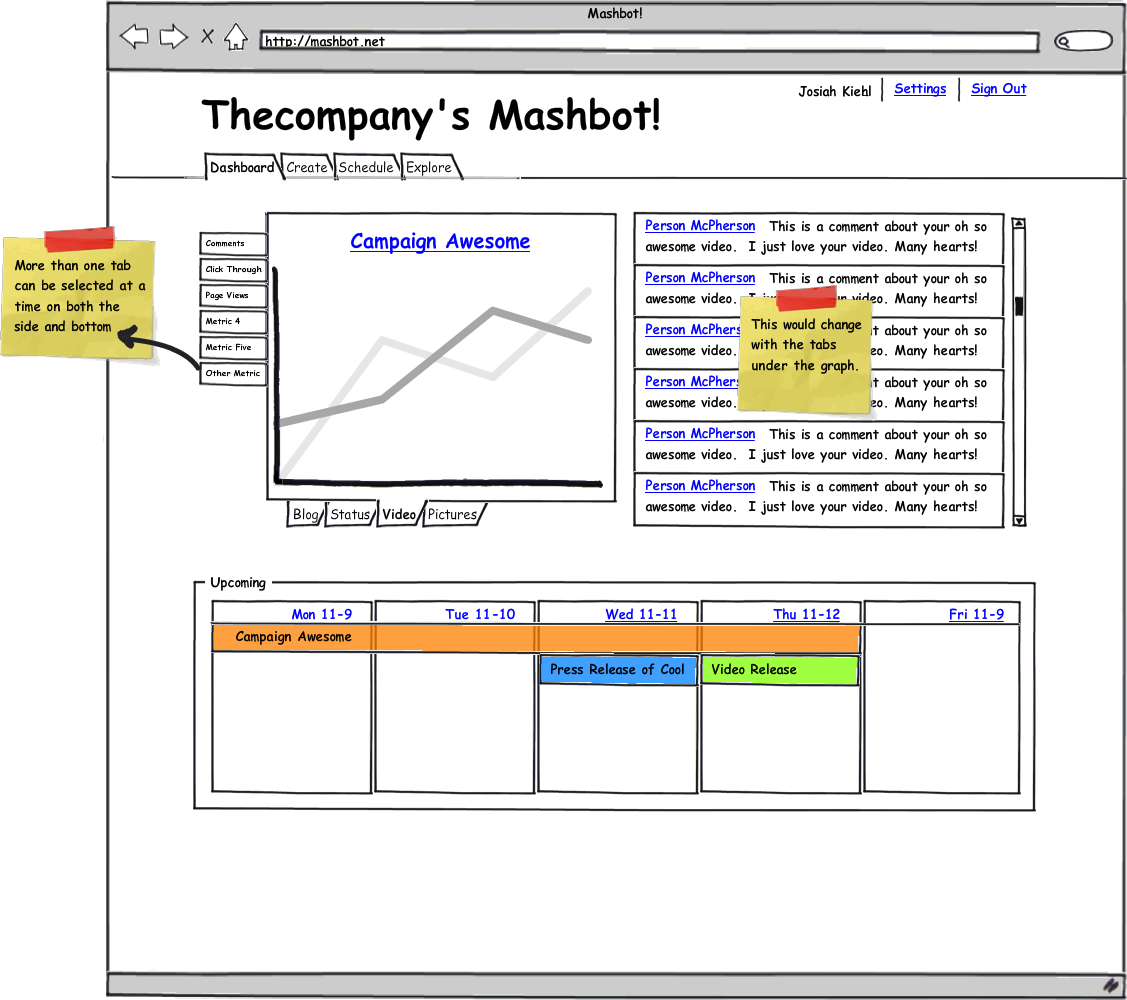
\includegraphics[width=7.5in]{../mockups/dashboard.png}
        \clearpage
        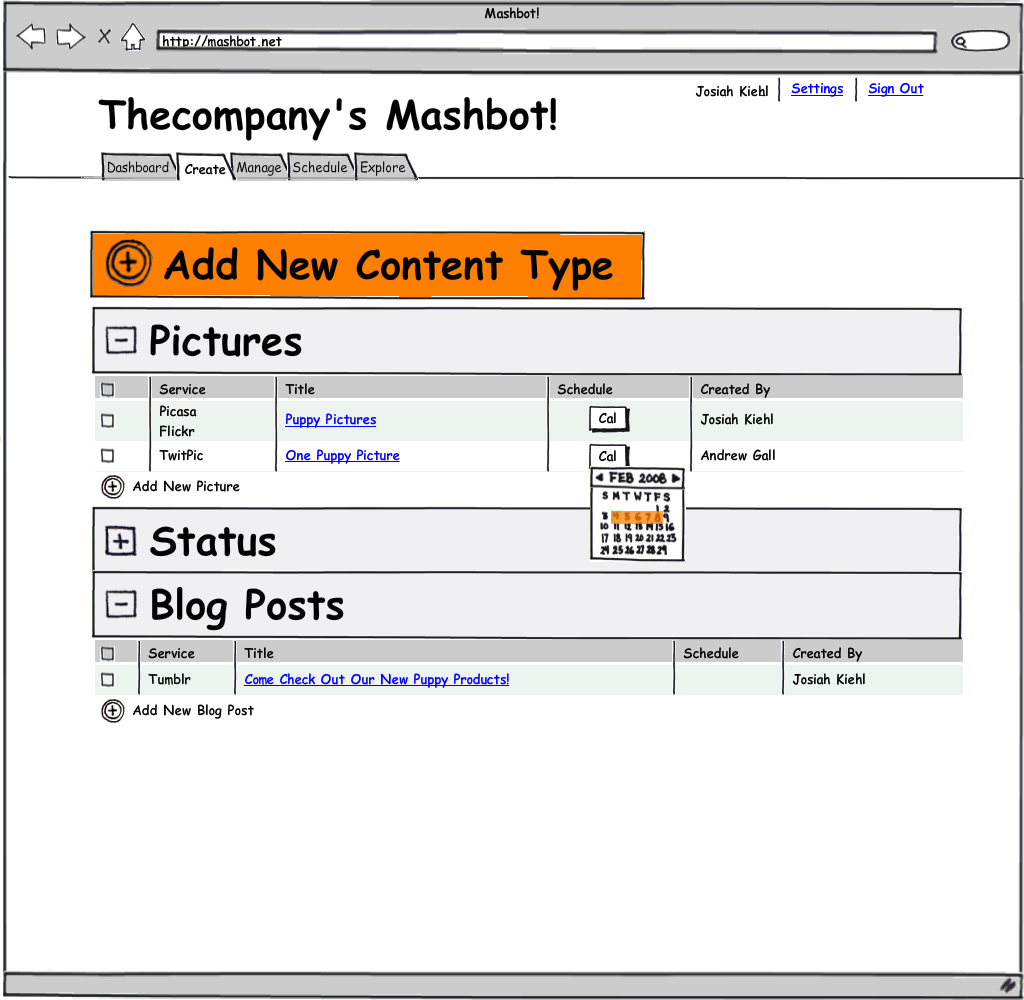
\includegraphics[width=7.5in]{../mockups/create.png}
        \clearpage
        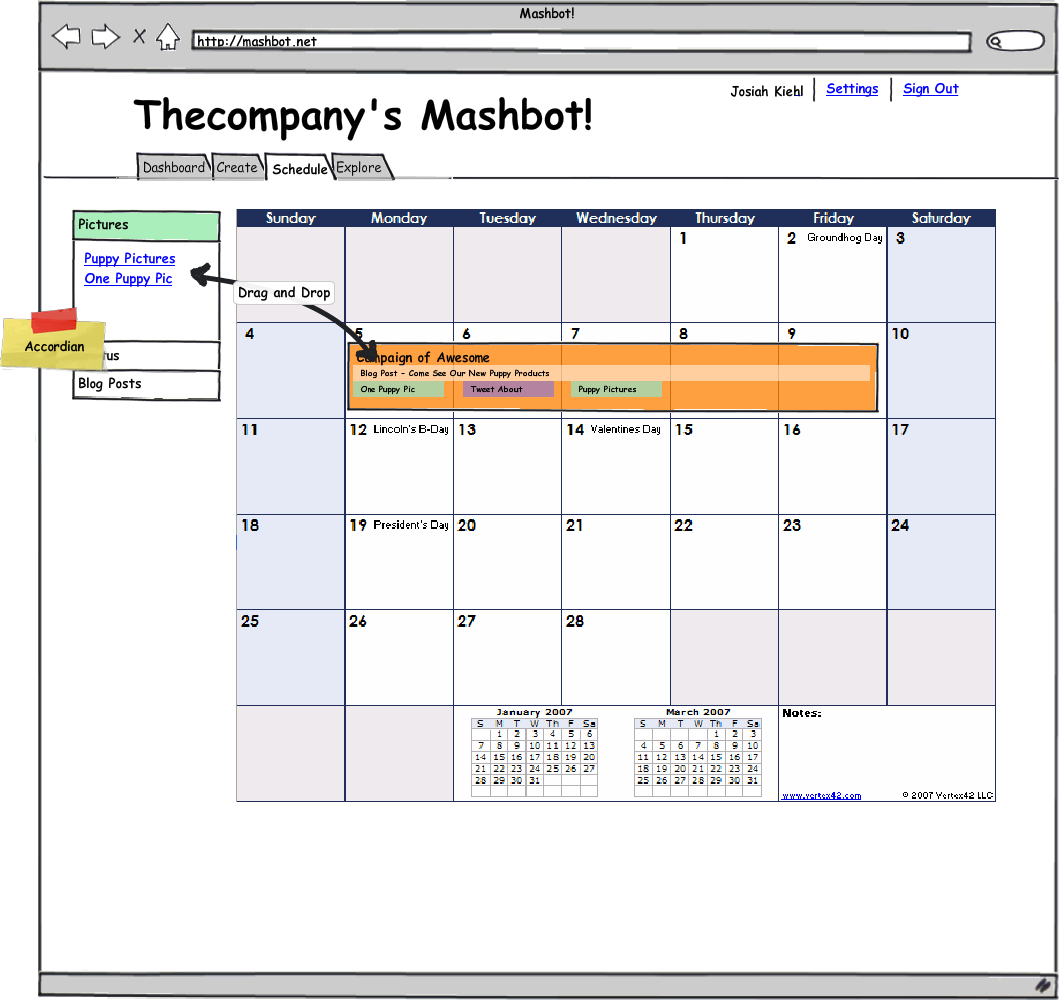
\includegraphics[width=7.5in]{../mockups/schedule.png}
        \clearpage
\section{Preliminary Analysis} % JK
Mashbot is a data driven web application.  It aggregates data from various web services.  This figure shows the flow of data through the web application.
There is a core that handles all requests for various data needed by the appluication.  Authentication information is retrieved from the database and used to request content from services.
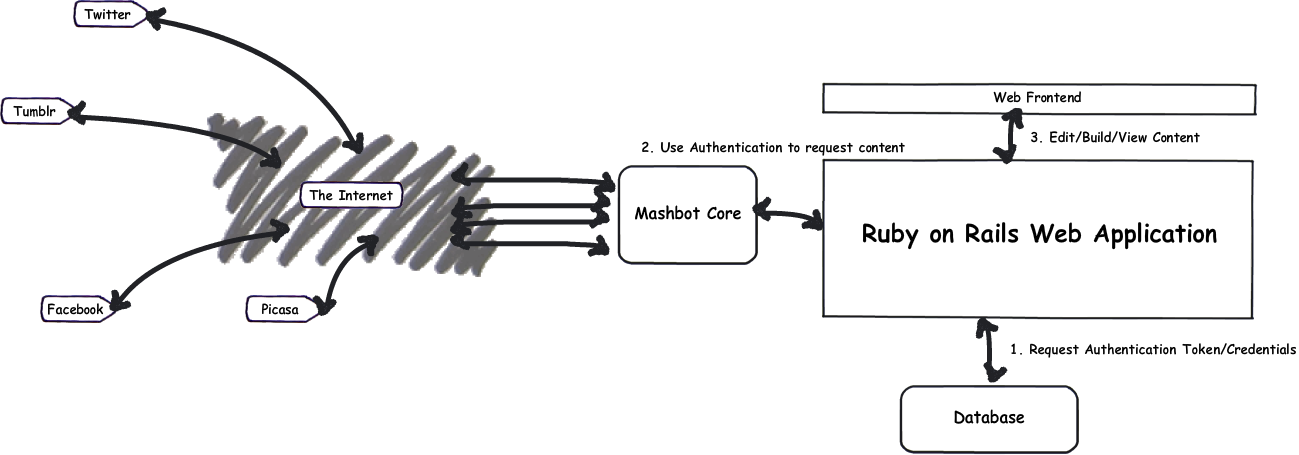
\includegraphics[width=7.5in]{../mockups/dataflow.png}
\section{Use Cases} % CR
  \begin{enumerate}
	\item A user should be able to register a new account
	\item A user should be able to log in
	\item A member should be able to log out
	\item A member should have a profile
	\item A member should be able to modify their profile
	\item A user's email should be verified when registering a new account.
	\item An admin should be able to modify accounts
	\item An admin should be able to suspend accounts
	\item An admin should be able to delete accounts
	\item A member should be able to monitor trending topics regarding their campaign
	\item A member should be able to monitor facebook groups related to campaigns
	\item A member should be able to view @replies to tweets related to their campaigns
	\item A member should be able to see responses to blog posts related to the campaign.
	\item An admin should be able to perform user account actions in bulk
	\item An admin should be able to see all campaigns
	\item An admin should be able to delete any campaign
	\item An admin should be able to edit all campaigns
	\item Mashbot campaigns! campaigns should allow multiple users to collaborate on a campaign
	\item Mashbot campaigns! should support multiple users
	\item A member should be able to store authentication for supported services
	\item A member should be able to add additional services to an existing campaign
	\item A member should be able to delete individual campaign elements 
	\item Members should have hierarchical permissions
	\item A campaign should have workflow approval process
	\item A member should be able to "unpublish" a campaign
	\item A member should be able to delete a campaign
	\item A member should be able to schedule events in bulk
	\item A member should be able to schedule "live dates" for individual 
	events.
	\item A member should be able to delete existing content from supported services
	\item A member should be able to see the content they have published in all supported services
	\item A member should be able to push to Facebook in a campaign
	\item A member should be able to post to a blog in a campaign
	\item A member should be able to post to Twitter in a campaign
	\item A member should be able to create a new campaign
	\item A member should get notified when activity occurs in a campaign they're working on
  \end{enumerate}

%% \section{IO}

%% Inputs
%%   CRUD
%%   Types
%%     Pictures
%%     Status/Tweet
%%     Blog
%%     Video

%% Users
%%   Name
%%   Email
%%   Company
%%   Permissions
%%   Accounts
    
%% Account
%%   What a company buys
%%   Allows user/campaign creation
  
%% Campaigns
%%   Name
%%   Schedule
%%   Content
%%     Distribution Channels


\end{document}


% LocalWords:  Mashbot
